\documentclass{scaffold/sigchi}
\usepackage{pifont} % Check marks
\newcommand{\cmark}{\ding{51}} % So we can use \cmark instead of \ding{51}
\newcommand{\xmark}{\ding{55}}
%\usepackage[none]{hyphenat}
\usepackage{makecell} % For table headers
\usepackage{multirow}

% \usepackage[style=numeric,sorting=nty, eprint=false,doi=true,isbn=false,url=false, maxbibnames=99, giveninits=false]{biblatex}
% \DeclareFieldFormat{labelnumberwidth}{#1\adddot\midsentence}

% \addbibresource{sample.bib}

% Title
\def\plaintitle{Impact of Audio and Visual Display of Positive Reinforcement on Supporting Habit Formation}
%\def\plaintitle{Investigating the Impact of Displaying Positive Reinforcement Using Different Modalities on Habit Formation}

% Authors as plain text
\def\plainauthor{First Author, Second Author, Third Author,
  Fourth Author, Fifth Author, Sixth Author}
\def\emptyauthor{}
\def\plainkeywords{habit formation; behaviour change; positive reinforcement}
\def\plaingeneralterms{Documentation, Standardization}
  \usepackage{pgfplots}
  \pgfplotsset{compat=1.12}

% Use this section to set the ACM copyright statement (e.g. for
% preprints).  Consult the conference website for the camera-ready
% copyright statement.

% Copyright
\CopyrightYear{2017}
%\setcopyright{acmcopyright}
\setcopyright{acmlicensed}
%\setcopyright{rightsretained}
%\setcopyright{usgov}
%\setcopyright{usgovmixed}
%\setcopyright{cagov}
%\setcopyright{cagovmixed}
% DOI
\doi{http://dx.doi.org/10.475/123_4}
% ISBN
\isbn{123-4567-24-567/08/06}
%Conference
\conferenceinfo{CHI'18,}{April 21--26, 2018, Montreal, Canada}
%Price
% \acmPrice{\$15.00}

% Use this command to override the default ACM copyright statement
% (e.g. for preprints).  Consult the conference website for the
% camera-ready copyright statement.

%% HOW TO OVERRIDE THE DEFAULT COPYRIGHT STRIP --
%% Please note you need to make sure the copy for your specific
%% license is used here!
% \toappear{
% Permission to make digital or hard copies of all or part of this work
% for personal or classroom use is granted without fee provided that
% copies are not made or distributed for profit or commercial advantage
% and that copies bear this notice and the full citation on the first
% page. Copyrights for components of this work owned by others than ACM
% must be honored. Abstracting with credit is permitted. To copy
% otherwise, or republish, to post on servers or to redistribute to
% lists, requires prior specific permission and/or a fee. Request
% permissions from \href{mailto:Permissions@acm.org}{Permissions@acm.org}. \\
% \emph{CHI '16},  May 07--12, 2016, San Jose, CA, USA \\
% ACM xxx-x-xxxx-xxxx-x/xx/xx\ldots \$15.00 \\
% DOI: \url{http://dx.doi.org/xx.xxxx/xxxxxxx.xxxxxxx}
% }

% Arabic page numbers for submission.  Remove this line to eliminate
% page numbers for the camera ready copy
% \pagenumbering{arabic}

% Load basic packages
\usepackage{balance}       % to better equalize the last page
\usepackage{graphics}      % for EPS, load graphicx instead 
\usepackage[T1]{fontenc}   % for umlauts and other diaeresis
\usepackage{txfonts}
\usepackage{mathptmx}
\usepackage[pdflang={en-US},pdftex]{hyperref}
\usepackage{color}
\usepackage{booktabs}
\usepackage{textcomp}

% Some optional stuff you might like/need.
\usepackage{microtype}        % Improved Tracking and Kerning
% \usepackage[all]{hypcap}    % Fixes bug in hyperref caption linking
\usepackage{ccicons}          % Cite your images correctly!
% \usepackage[utf8]{inputenc} % for a UTF8 editor only

% If you want to use todo notes, marginpars etc. during creation of
% your draft document, you have to enable the "chi_draft" option for
% the document class. To do this, change the very first line to:
% "\documentclass[chi_draft]{sigchi}". You can then place todo notes
% by using the "\todo{...}"  command. Make sure to disable the draft
% option again before submitting your final document.
\usepackage{todonotes}






% llt: Define a global style for URLs, rather that the default one
\makeatletter
\def\url@leostyle{%
  \@ifundefined{selectfont}{
    \def\UrlFont{\sf}
  }{
    \def\UrlFont{\small\bf\ttfamily}
  }}
\makeatother
\urlstyle{leo}




% To make various LaTeX processors do the right thing with page size.
\def\pprw{8.5in}
\def\pprh{11in}
\special{papersize=\pprw,\pprh}
\setlength{\paperwidth}{\pprw}
\setlength{\paperheight}{\pprh}
\setlength{\pdfpagewidth}{\pprw}
\setlength{\pdfpageheight}{\pprh}

% Make sure hyperref comes last of your loaded packages, to give it a
% fighting chance of not being over-written, since its job is to
% redefine many LaTeX commands.
\definecolor{linkColor}{RGB}{6,125,233}
\hypersetup{%
  pdftitle={\plaintitle},
% Use \plainauthor for final version.
%  pdfauthor={\plainauthor},
  pdfauthor={\emptyauthor},
  pdfkeywords={\plainkeywords},
  pdfdisplaydoctitle=true, % For Accessibility
  bookmarksnumbered,
  pdfstartview={FitH},
  colorlinks,
  citecolor=black,
  filecolor=black,
  linkcolor=black,
  urlcolor=linkColor,
  breaklinks=true,
  hypertexnames=false
}

% create a shortcut to typeset table headings
% \newcommand\tabhead[1]{\small\textbf{#1}}

\title{\plaintitle}



\usetikzlibrary{patterns}
% Authors on paper
\numberofauthors{3}
\author{%
  \alignauthor{Leave Authors Anonymous\\
    \affaddr{for Submission}\\
    \affaddr{City, Country}\\
    \email{e-mail address}}\\
  \alignauthor{Leave Authors Anonymous\\
    \affaddr{for Submission}\\
    \affaddr{City, Country}\\
    \email{e-mail address}}\\
  \alignauthor{Leave Authors Anonymous\\
    \affaddr{for Submission}\\
    \affaddr{City, Country}\\
    \email{e-mail address}}\\
}

\begin{document}

\maketitle

\begin{abstract}
Habit formation technologies use rewards and points as means for providing positive reinforcement, often in visual or audio forms such as jingles, badges or animations. Providing appropriate rewards increases the chances for developing a new habit; yet, research on how these rewards should be delivered and the impact that this has on the process of habit formation is scarce. In this paper, we investigate how three types of positive reinforcement (audio, visual, audio-visual) influence habit completion and automaticity. We describe a four week study in which participants used a chatbot that delivered different types of rewards for completing a new daily habit. The results reported higher habit completion rates when a reward was present, especially for the audio-visual condition, without necessarily increasing behaviour automaticity. This has implications for the design of habit formation technologies that rely on audio and visual rewards as means of positive reinforcement.
\end{abstract}

\category{H.5.m}{Information interfaces and 
presentation (e.g. HCI)}{Miscellaneous}
\category{H.5.2}{User Interfaces}{User-Centered Design}

\keywords{\plainkeywords}


\section{Introduction}
%In recent years, d
Designing technology to support habit formation has become an important theme in HCI research. This is not surprising, as a good understanding of how to design systems that support habit development helps to ensure that they lead to long lasting changes in one's behaviour~\cite{how_to_evaluate_tech_for_behaviour_change}. %While there is evidence that  supporting contextual cues, regular repetition and positive reinforcement facilitates the formation of new habits~\cite{article_beyond_self_tracking_designing_apps}, %there is little research into 
%the impact that different types of positive reinforcement have on habit formation remains largely unexplored \textbf{[insert refs to papers that do look at this her, OM]}.
%
%Positive reinforcement plays an important role in habit formation. It is used as a reward to reinforce a habit and increase repetition~\cite{positive_reinforcement_pro}. 
%
Rewards play an important part in supplementing the positive reinforcement necessary for habit forming processes~\cite{positive_reinforcement_pro}. An example of this in habit formation technologies is the use of coins and points as rewards to increase task repetition. However, studies have shown that this form of extrinsic rewards can also reduce motivation and therefore hinder habit formation in the long run~\cite{article_meta_analytic_review_intrinsic_motivation}.

%While habit formation technologies use extrinsic rewards to increase task repetition, such as coins and points, studies have shown that extrinsic rewards can reduce motivation and therefore hinder habit development~\cite{article_meta_analytic_review_intrinsic_motivation}. 
%

Other types of positive reinforcement include sending text messages to affirm behaviour~\cite{chi_crowd_designed_motivation} and coaching a person throughout the habit formation process~\cite{coaching_not_that_good}. But these approaches have been shown to encourage repetitive action and dependency, rather than automaticity of behaviour that is characteristic of habits~\cite{habits_as_automaticity_not_frequency_gardner}.
%
An alternative approach is to provide intrinsic, rather than extrinsic, motivation after a habit is completed~\cite{article_a_self_efficacy, article_meta_analytic_review_intrinsic_motivation}. Intrinsic motivation refers to behaviour that is driven by internal rewards that focus on increasing personal motivation to complete a task, such as health benefits, as opposed to, for example, monetary extrinsic rewards.

When delivered through technology, positive reinforcement aimed at facilitating intrinsic motivation is predominantly presented in a form of visual feedback, e.g. %positive messages
~\cite{comparison_of_auditory_visual_feedback, visual_mode_better, article_realtime_feedback_improving_medication_taking}. 
%
However, with the advent of ubiquitous and mobile technologies, visual feedback may not always be an appropriate form of presenting rewards, e.g. when a display is not visible or even not available.  Alternative non-visual displays have been used to overcome these issues in a number of other applications (e.g.~\cite{burke2006comparing, vazquez2012auditory, chi_oussama_tap_the_shapetones}), 
%Audio for example have been shown to compliment visual displays in situations where vision alone is unreliable. 
%Research investigating non-visual display of rewards is scarce, and 
but the benefits of non-visual feedback as a form of positive reinforcement in the context of habit formation have received limited attention.


%however only as a means to increase task performance; 
%
%research investigating the use of other modes for habit formation is scarce. 
%
%Although auditory feedback has been shown to improve task performance~(e.g.~\cite{burke2006comparing, vazquez2012auditory, chi_oussama_tap_the_shapetones}), it is not known how it affects habit formation.

%Sending positive text messages to affirm behaviour is one type of positive reinforcement that aims to motivate habit completion~\cite{chi_crowd_designed_motivation}. However, this may simply encourage repetitive actions rather than help to develop automaticity of behaviour that characterises habits~\cite{habits_as_automaticity_not_frequency_gardner}. Coaching a person throughout the habit formation process by guiding them every step of the way encourages habit performance~\cite{coaching_not_that_good}, but can also build dependency when the coach is removed~\cite{article_dont_kick_habit, article_realtime_feedback_improving_medication_taking}. A successful method of positive reinforcement is to build habit automaticity, rather than repetitive actions~\cite{article_beyond_self_tracking_designing_apps}, which can be helped by using intrinsic motivation after a habit is completed~\cite{article_a_self_efficacy, article_meta_analytic_review_intrinsic_motivation}.

%When delivered through technology, positive reinforcement aimed at facilitating intrinsic motivation is usually presented in a form of visual feedback~\cite{comparison_of_auditory_visual_feedback, visual_mode_better, article_realtime_feedback_improving_medication_taking}, however only as a means to increase task performance; research investigating the use of other modes for habit formation is scarce. Although auditory feedback has been shown to improve task performance~(e.g.~\cite{burke2006comparing, vazquez2012auditory, chi_oussama_tap_the_shapetones}), it is not known how it affects habit formation.

% The type of intrinsic reward for habit formation has had little research improves motivation to complete a habit, even when the reward is removed~\cite{article_meta_analytic_review_intrinsic_motivation}.

% Motivation can be encouraged by giving people positive reinforcement rewards after they complete an action~\cite{positive_reinforcement_pro}. However, how the reward is delivered and the type of reward used is also crucial to success.

%The method of delivery should suit each individual user and a choice of delivery should be available. For example, a survey on feedback systems~\cite{article_user_centred_multimodal_reminders} advised that delivery of interaction should span different modalities to increase retention and better suit the needs of users. Although interaction across modalities is important, this research does not have configurable feedback, but aims to compare how each type of feedback can affect motivation. Monetary (extrinsic) rewards can hinder motivation~\cite{article_meta_analytic_review_intrinsic_motivation}, whereas, satisfaction-based (intrinsic) rewards can be beneficial to motivation and should be preferred. 
%This study uses a chatbot to deliver intrinsic positive reinforcement rewards from different modalities to see how participants habit automaticity and performance are affected.

To explore the potential of non-visual feedback in supporting new habits, we conducted a 4-week situated study that explored the impact of different types of positive reinforcement (audio, visual, audio-visual) on the process of habit formation.
The main contribution of our work is a better understanding of how these types of positive feedback affect the development of new habits. We show that combined audio-visual positive reinforcement is more effective at supporting repetition and habit completion compared to visual- or audio-only displays. However, it does not seem to affect habit automaticity.
%
This has implications for the design of habit formation technologies that rely on audio and visual rewards as means of positive reinforcement.

\section{Background}
\subsection{Role of positive reinforcement in habit formation}
Changing behaviour permanently requires forming a new habit~\cite{article_experiences_of_habit_formation}, which in turn depends on consistent repetition~\cite{article_how_habits_formed_modelling_habit_formation}. The easier the action, the shorter the time before it turns into a habit. For example, tasks as simple as drinking water may require 18 days to become automatic, but for going to the gym that period may as well take 254 days~\cite{article_how_habits_formed_modelling_habit_formation}. To ensure this process is shorter, the new habit should be linked with a regularly occuring event. Building the habit around an existing routine facilitates repetition~\cite{habits_event_cues_1}, as the task that is already a part of daily routine and the context in which it takes place both serve as  triggers to action~\cite{habits_event_cues_2}. Such event-based, contextual cues also make it easier to remember to repeat the task~\cite{article_implementation_intentions_multicue, article_implementation_intentions}.
%due to change in time with change in environment, e.g. the weekend~\cite{coaching_not_that_good}. Event-based cues help connect the contextual information with the action and builds habit automaticity~\cite{article_implementation_intentions}.

Motivation further supports the process of habit formation. Positive reinforcement at the end of the task rewards the person by encouraging them to perform the action again, until it becomes habitual~\cite{article_a_self_efficacy}. The reward increases intrinsic motivation by inducing the feeling of satisfaction~\cite{article_promoting_habit_formation} and increasing the person's perception of their performance~\cite{positive_reinforcement_pro}, especially when the task itself is interesting~\cite{article_meta_analytic_review_intrinsic_motivation}. Therefore, when designing behaviour change technology, the delivery of the reward must be carefully considered because it can affect the formation of new habits.

\subsection{Providing positive reinforcement with technology}
Smartphone apps are often used to support the process of habit formation~\cite{survey_on_current_apps_of_steel}. However, even though most of them are highly rated, they are not grounded in theory~\cite{article_beyond_self_tracking_designing_apps, article_dont_kick_habit}. Moreover, several studies suggest that users may become dependent on the app and the behaviour is not sustained after the app is removed~\cite{survey_on_apps_2,article_dont_kick_habit,article_realtime_feedback_improving_medication_taking}, due to the lack of automaticity developed during the habit tracking process. 
%This can be a problem when using mobile apps to consistently manage behaviour and can create a notable difference in the persons behaviour after it is removed~\cite{article_my_phone_is_part_of_my_soul}. 
Building habit automaticity, while avoiding developing dependency is therefore key, but requires the desired action to be built around an existing routine~\cite{article_how_habits_formed_modelling_habit_formation, article_implementation_intentions_multicue}. Technology should help with routine creation by having additional checks to guard against changes in routine that check in with people about their habit if their situation changes~\cite{article_dont_forget_your_pill}. While this could be facilitated by apps (e.g. see~\cite{article_beyond_self_tracking_designing_apps}, there are other possibilities.

Chatbots are becoming increasingly popular. They have been integrated into messaging apps, such as the \textit{Telegram} app to track food habits~\cite{telegram_bot_tracking_habits} and are seen as a significant component of HCI's increasing shift towards new interaction paradigms involving natural language user interfaces~\cite{chatbots_and_new_world_of_hci}. Applying the design guidelines for building habit formation systems~\cite{article_beyond_self_tracking_designing_apps} to a chatbot presents a new opportunity for delivering positive reinfocement.

%, recommend avoiding features that teach users to rely on technology and use trigger events to help monitor behaviour. These messages check after an existing routine to see if the task was completed. Combining these guidelines with a chatbot presents a rare method of delivering positive reinforcement.

Positive reinforcement rewards can be delivered via different modalities; audio, visual and audio-visual modes are common choices~\cite{desinging_interface_speech_tech}. For example, audio feedback has been shown to improve task success when used as a notification for a task~\cite{auditory_notifications_increase_delivery_success}, but little research has looked at its impact on the completion of habits. On the other hand, fast visual feedback has been shown to be preferred over audio when the relative importance of the task is high~\cite{visual_mode_better} and to improve the consistency of a medication-taking habits~\cite{article_realtime_feedback_improving_medication_taking}. However, when the visual feedback is removed, the performance can drop, which suggests a dependency on the technology and the visual feedback it provides. 
%Instead these cues should be constructed around another routine to build habit automaticity and allowing for permanent behaviour change after the system is removed. 
Although audio and visual feedback has been shown to improve task performance, the combination of both tends to be more effective than audio or visual alone~\cite{benefits_of_audio_visual_1, benefits_of_audio_visual_2, chi_oussama_tap_the_shapetones}. For example, a meta-analysis of 43 multi-modal studies~\cite{comparing_modalities_effects_of_visual_auditory} revealed that a combined audio-visual modality was the most effective at increasing performance of a single task, compared with only visual or only audio feedback. However, care needs to be taken when adding an extra modality: this study also showed that while visual feedback improved task performance, it reduced task quality~\cite{comparing_modalities_effects_of_visual_auditory}.

Overall, there is evidence that these three types of feedback increase task completion in different ways. However, how -- and whether -- this type of feedback influences habit formation is unclear. Therefoe, below we describe an in-the-wild study that explored how audio, visual and audio-visual positive reinforcement influences habit formation.

\begin{figure}
  \centering
  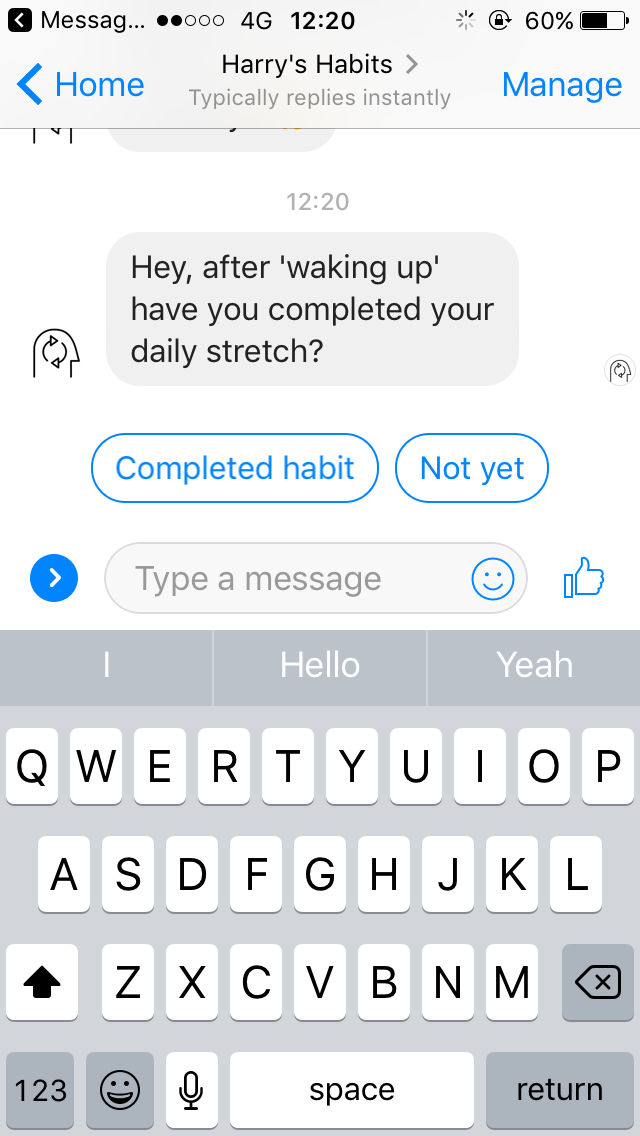
\includegraphics[width=0.47\columnwidth]{figures/reminder.png}
  \hspace{5px}
  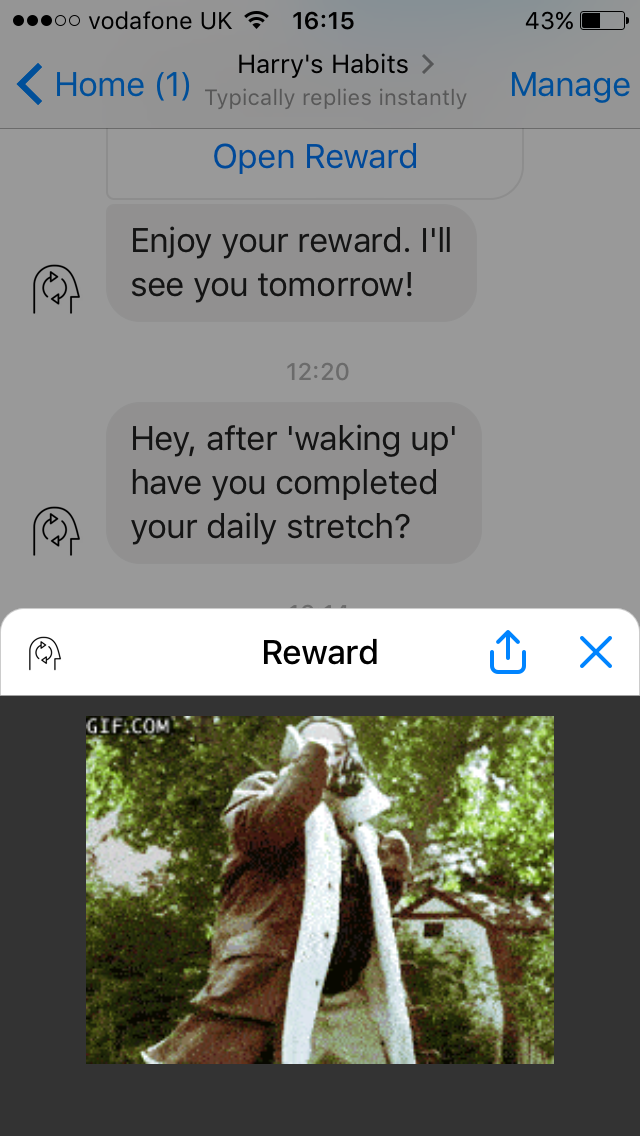
\includegraphics[width=0.47\columnwidth]{figures/reward-visual.png}
  \caption{Bot's ``check in'' message (left) and an example of a reward (right).}~\label{fig:setup}
\end{figure}

\section{Comparing Types of Positive Reinforcement}
The aim of the study was to explore what type of positive reinforcement (audio, visual, audio-visual) would be the most effective in supporting regular habit completion and the development of automaticity. We conducted a 4-week situated study followed by optional semi-structured interviews to evaluate each mode of reward. Positive reinforcement was delivered by a chatbot.

\subsection{Method}
For the purpose of the study, we developed a chatbot that was used to deliver positive reinforcement to participants wanting to start a new healthy habit. To ensure they were motivated to pursue their habit, we gave them a choice: they could select a physical activity habit (stretching, press ups, the plank) or a relaxing habit (reading, writing, meditation). We selected these specific habits, as they are easy to complete and generally do not require any special equipment. Moreover, simple tasks become automatic quicker than complex actions~\cite{article_how_habits_formed_modelling_habit_formation} and such simple habits allow to observe changes in automaticity of behaviour within four weeks~\cite{article_beyond_self_tracking_designing_apps}. 
The study was approved by the University Ethics Committee.

\subsubsection{Participants}
Fifty-four participants were recruited on social networks. They were 18-63 years old (mean age=26.7 years old, SD=10); 32 (59\%) were men, 14 (26\%) were women, and eight (15\%)  chose not to disclose their gender; 16 (29\%) were university students. As their habit of choice, 15 participants selected meditation, 12 selected stretching, 11 selected press ups, six selected reading, five selected writing and other five selected the plank. In terms of interactions with the bot, 21 participants used a web browser, 18 used iOS devices, 12 used Android and three used another mobile device. 

\begin{table}
  \centering   
  \begin{tabular}{l l l}
    % \toprule
\multicolumn{1}{l}{\small \textit{Condition}} &
\multicolumn{1}{p{1.4cm}}{\small \textit{Number of Participants}} &
\multicolumn{1}{l}{\small \textit{Positive Reinforcement}} \\
    \midrule
    Audio & 14 & 15s audio\\
    Visual & 15 & 15s GIF \\
    Audio-Visual & 14 & 15s GIF and audio \\
    None (control group) & 11 & Confirmation \\
    % \bottomrule
  \end{tabular}
  \caption{Study conditions and their corresponding types of positive reinforcement.}~\label{table:precise_rewards}
\end{table}

\subsubsection{Design}
Participants were randomly assigned to one of four conditions: Audio, Visual, Audio-Visual and the Control group. Each condition differed by the type of positive reinforcement it provided after participants reported completion of their daily habit: participants in the Audio condition received a fifteen-second audio clip as a reward for completing their habit; in the Visual condition they received a fifteen-second GIF; the Audio-Visual condition combined the audio clip with a GIF; and participants in the Control group received a confirmation message (``Thanks.''). Study conditions are summarised in Table~\ref{table:precise_rewards}. 

For each condition, we measured the number of times the selected habit was completed during the study. ``Habit completion rate'' was defined as the number of times the person repeated and reported the behaviour, divided by 21 days during which participants interacted with the bot. We also measured the change in automaticity of the behaviour during the final weeks, to assess habit strength.



\subsubsection{Materials}
To deliver different types of positive reinforcement, we built a custom Facebook Messenger bot (see Figure~\ref{fig:setup}). Bot's functionality and approach to support habit formation was informed by~\cite{article_beyond_self_tracking_designing_apps}: rather than providing reminders, the bot first allowed participants to define a routine and during the study provided ``check in'' notifications to see if the routine was followed; if the routine was not working and participants did not complete their habit on time, the bot then suggested changes to the plan. For example, if a participant regularly snoozed the check in notification, the bot would ask if they wanted to move the check in time for later in the day.

We decided to use a bot as it can easily send notifications, is cross-platform and thus highly available, and also offers simple user interface and easy interactions already familiar to the users. Moreover, the integration with the platform meant that interactions with the bot would be visible alongside participant's other conversations, making it easier to report completion of the habit~\cite{the_power_of_logging_mobile_notifications}.

As the aim of the rewards was to motivate the participants to keep coming back every day and completing their habits, we identified several ``motivational'' GIFs and audio files, and each GIF file was tweaked to match the audio frequency. We decided to use popular GIFs with internet memes, i.e. content that is passed along from person to person via social media posts~\cite{meme_definition}. Humorous GIF memes make people laugh and are popular on some social media sites, where they usually are the most engaging content~\cite{meme_gifs_are_good}. Given that our bot was integrated with Facebook, and that Facebook introduced built-in support for animated GIFs~\cite{fb_gif_rollout}, memes would integrate well with the bot environment. 

We also used the bot to collect responses to the Self-Report Behavioural Automaticity Index (SRBAI;~\cite{article_4q_SRBAI}). This is a validated four-item instrument for measuring habit automaticity, which can be used as an indicator of habit strength. %SRBAI statements are presented on a 5-point Likert scale with answers from 'Strongly Disagree' (1) to 'Strongly Agree' (5); higher scores indicate higher self-reported levels of automaticity.

\begin{figure}
  \centering
  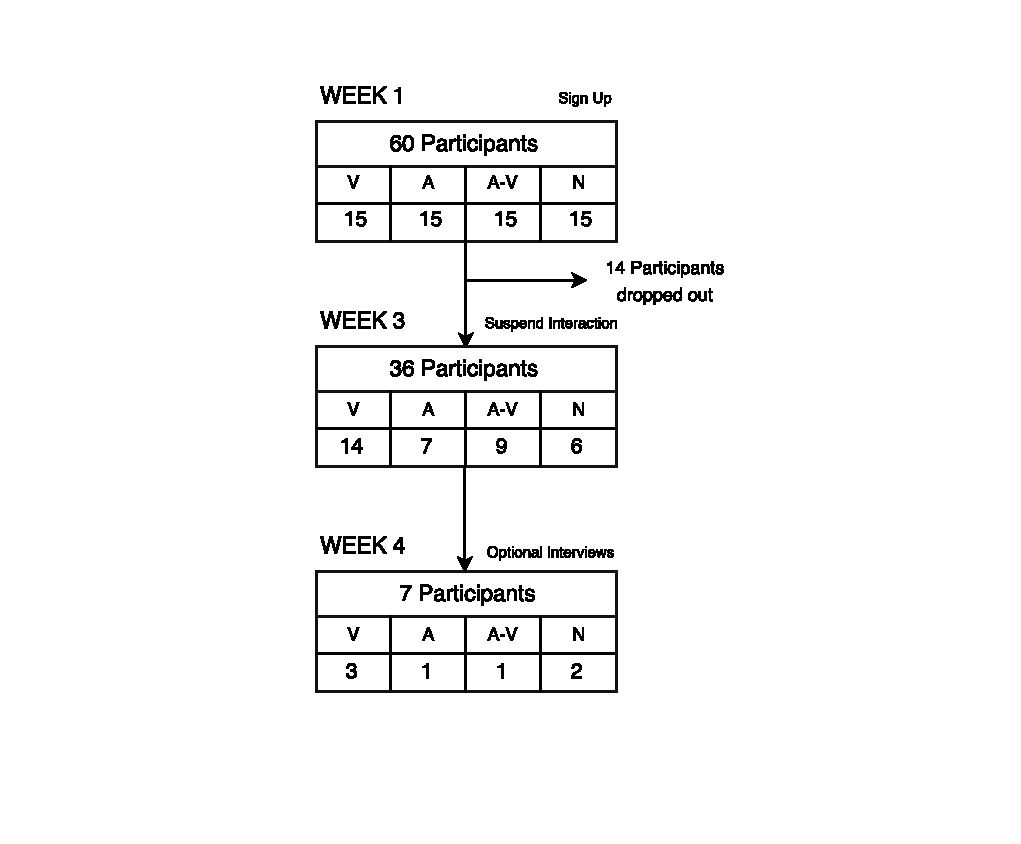
\includegraphics[width=0.7\columnwidth]{figures/study-flow.pdf}
  \caption{Participant drop-out during the four-week study. A: audio, V: visual, A-V: audio-visual, N: no reward.}~\label{fig:study_dropout}
\end{figure}

\subsubsection{Procedure}
Recruitment posts instructed potential participants to connect with our bot via Facebook Messenger. By connecting with the bot, completing the set-up and providing demographic information, participants expressed their consent to participate in the study.

During the set-up process, participants were asked to select one of the healthy habits they would like to develop and, as recommended in~\cite{article_dont_forget_your_pill} for technologies supporting habit formation, to specify contextual cues associated with that habit and the time they would want to complete it (morning, afternoon, evening). Once their habit routine was specified, participants were automatically assigned to one of the study conditions. 

Next, for the first three weeks of the study, participants were asked to complete their chosen habit as part of the specified routine. During that period, the bot ``checked in'' with the participants after their specified time (see Figure~\ref{fig:setup}, left). Participants then could indicate whether they completed the habit or not. If they reported habit completion, they would receive their positive reinforcement message (see Figure~\ref{fig:setup}, right). If they selected ``not yet'', the bot would check on the participant again an hour later. This allowed for the checks to be snoozed, to ensure the new habit fits into participant's routine. If participants constantly told the bot they had not completed their habit yet, the bot would suggest making changes to the routine. Throughout the study, information about how well each participant was performing was not revealed, as streaks can provide extrinsic motivation~\cite{article_dont_kick_habit}, which might have confouded our results. 

After interacting with the bot for three weeks, participants were asked to complete the SRBAI questionnaire and answer a set of questions about the positive reinforcement they received (e.g. how useful it was, whether they liked it). Next, during the final week of the study, bot interactions were suspended, but participants were still asked to continue with their habit. At the end of that period, participants were asked to complete the SRBAI questionnaire again along with a few questions about their experience with the rewards. 

Participants also had an option to opt-in for an interview to discuss their experience. The interviews were conducted after the 4-week study and explored participants experience with trying to maintain their habit after the interactions with the bot ended, their attitudes towards positive reinforcement and towards the bot itself.

%\subsubsection{Analysis}
%The results are grouped into two measurements habit completion and habit automaticity. For each measurement three categories are used for comparison: i) The effect of each condition on habit completion ii) The rewards effect on habit completion, iii) Multiple vs. single-mode feedback on habit completion. Participants also had an option to opt-in for an interview to discuss their experience. The interviews were conducted after the four-week study and explored participants experience with trying to maintain their habit after the interactions with the bot ended, their attitudes towards positive reinforcement and towards the bot itself. 

\section{Results}
Thirty-six participants completed the study (see Figure~\ref{fig:study_dropout}); seven of them were from the Audio condition, 14 from the Visual condition, nine were from Audio-Visual and six from the Control group. They were 18-63 years old (mean=27 years old, SD=12); 23 (64\%) were men, 11 (30\%) were women and two (6\%) didn't disclose their gender. 

Among participants who completed the study, meditation was the most popular habit (12 participants, or 33\%), followed by press ups (eight participants, or 22\%), then stretching (six participants, or 15\%). Reading and writing were the least common, only selected by four (11\%) and two (5\%) participants, respectively.



\begin{figure}
\centering
 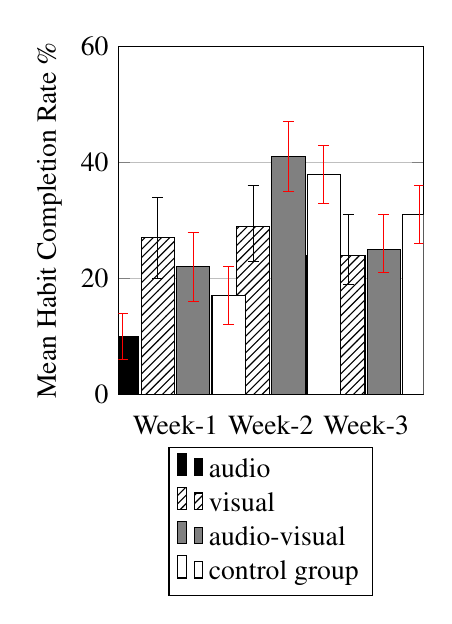
\begin{tikzpicture}
   \begin{axis}[
      width  = 0.45*\textwidth,
      height = 6cm,
      major x tick style = transparent,
      ybar=2*\pgflinewidth,
      bar width=12pt,
      ymajorgrids = true,
      symbolic x coords={Week-1, Week-2, Week-3},
      xtick = data,
      scaled y ticks = false,
      enlarge x limits=0.3,
      ymin=0,
      ymax=60,
      legend cell align=left,
      legend style={at={(0.5,-0.15)},anchor=north},
      ylabel={Mean Habit Completion Rate \%},
   ]
   
      \addplot[style={fill=black},error bars/.cd, y dir=both, y explicit,error bar style=red]
           coordinates { % Audio
          (Week-1, 10)  += (0,4) -= (0,4)
          (Week-2, 0)+= (0,4) -= (0,0.5)
          (Week-3, 24)+= (0,4) -= (0,4)
           };


      \addplot[style={fill=white},  postaction={
        pattern=north east lines
    }, error bars/.cd, y dir=both, y explicit]
          coordinates { % Visual
          (Week-1, 27)  += (0,7) -= (0,7)
          (Week-2, 29) += (0,7) -= (0,6)
          (Week-3, 24) += (0,7) -= (0,5)
      };


      \addplot[style={fill=gray},error bars/.cd, y dir=both, y explicit,error bar style=red]
           coordinates {  % audio-visual
          (Week-1, 22) += (0,6) -= (0,6)
          (Week-2, 41)+= (0,6) -= (0,6)
          (Week-3, 25)+= (0,6) -= (0,4)
      };
           
      \addplot[style={fill=white},error bars/.cd, y dir=both, y explicit,error bar style=red]
           coordinates { % Control
          (Week-1, 17)+= (0,5) -= (0,5)
          (Week-2, 38)+= (0,5) -= (0,5)
          (Week-3, 31) += (0,5) -= (0,5)
      };
      \legend{audio, visual, audio-visual, control group}

  \end{axis}
  \end{tikzpicture}
  \caption{The effect of each condition on habit completion.}~\label{fig:habit_completion_1}
\end{figure}


\subsection{Habit Completion}
% Habit completion Rate= (SUM of habits-completed for condition / 21 (days)) * 100%
% Avg Rate per week = (SUM of habits-completed for condition / <number of people in condition> / 7 (days)) * 100%
Overall, completion rates varied from 5\% to 100\% across individual participants (mean=30\%). The average habit completion rate was the highest for the Audio-Visual condition, with 33\%, followed by 29\% for the Visual condition, 28\% for the control condition and the lowest for Audio, with 14\%. Figure~\ref{fig:habit_completion_1} shows the average completion rate on a weekly basis for all conditions.


\begin{figure}
  \centering
 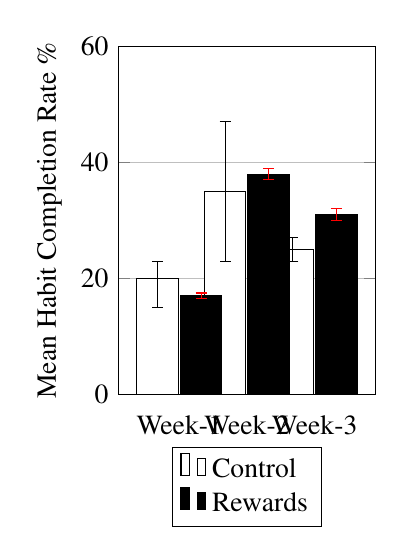
\begin{tikzpicture}
   \begin{axis}[
      width  = 0.4*\textwidth,
      height = 6cm,
      major x tick style = transparent,
      ybar=2*\pgflinewidth,
      bar width=15pt,
      ymajorgrids = true,
      symbolic x coords={Week-1, Week-2, Week-3},
      xtick = data,
      scaled y ticks = false,
      enlarge x limits=0.45,
      ymin=0,
      ymax=60,
      legend cell align=left,
      legend style={at={(0.5,-0.15)},anchor=north},
      ylabel={Mean Habit Completion Rate \%},
   ]
      \addplot[style={fill=white},error bars/.cd, y dir=both, y explicit]
          coordinates { % Rewards
          (Week-1, 20) += (0,3) -= (0,5)
          (Week-2, 35) += (0,12) -= (0,12)
          (Week-3, 25) += (0,2) -= (0,2)
          };

      \addplot[style={fill=black},error bars/.cd, y dir=both, y explicit,error bar style=red]
           coordinates {  % Control group
     	  (Week-1, 17) += (0,0.5) -= (0,0.5)
          (Week-2, 38) += (0,0.9) -= (0,0.9)
          (Week-3, 31) += (0,1) -= (0,1)
           };

      \legend{Control, Rewards}

  \end{axis}
  \end{tikzpicture}
  \caption{The rewards effect on habit completion.}~\label{fig:habit_completion_2}
\end{figure}

\subsubsection{The effect of each condition on habit completion}
To investigate the levels of habit completion per condition, we conducted a one-way ANOVA across each week. The analysis (see Figure~\ref{fig:habit_completion_1}) revealed that there was a statistically significant difference between each reward ($F(2,624) = 27.007$, $p < 0.05$). A Tukey post hoc test revealed that the Audio ($0.081 + 0.274$, $p < 0.005$), Control ($0.182 + 0.386$, $p < 0.005$) and Visual ($0.267$ + $0.484$, $p = 0.025$) feedback conditions were significantly lower when compared to the Audio-Visual ($0.373$ + $0.484$, $p < 0.005$) condition.




\subsubsection{The rewards effect on habit completion}
To explore the effect of rewards on the number of habits completed, compared with the control group, a one-way between-groups ANOVA with planned comparisons was conducted (see Figure~\ref{fig:habit_completion_2}). Participants were divided into two groups: group one with rewards, group two without rewards. There was a statistically significant difference at the $p$ $<$ $0.005$ level in both groups for week one and three: week one, $F(1,23.20) = 9.48$, $p = 0.005$, week two, $F(1,33.35) = 4.46$, p = 0.42 and week three, $F(1,0) = 17.01$, $p\leq 0.005$. The effect size for week one, week two and week three are large, calculated using $\eta^{2}$, were 0.25, 0.39 and 0.43 respectively, reporting a large difference in the mean scores.


\subsubsection{Multiple vs. single-mode feedback on habit completion}
The results from our study report a significant increase in habit completion for multiple modes (audio-visual). The significance of this finding was tested by conducting a one-way between-groups ANOVA with planned comparisons (see Figure~\ref{fig:habit_completion_3}). Participants were divided into two groups according to their mode. Group one: audio rewards and visual rewards, group two: audio-visual rewards. There was a statistically significant difference between groups each week ($p$ $<$ $0.005$) week one, $F(1,50) = 0.69$, $p = 0.410$, week two, $F(1,50) = 23.04$, $p$ $<$ $0.005$ and week three, $F(1,50) = 8.85$. The effect size for week one, week two and week three are large, calculated using $\eta^{2}$, were 0.25, 0.39 and 0.43 respectively, reporting an increasing difference in the mean scores throughout weeks.



\begin{figure}
  \centering
 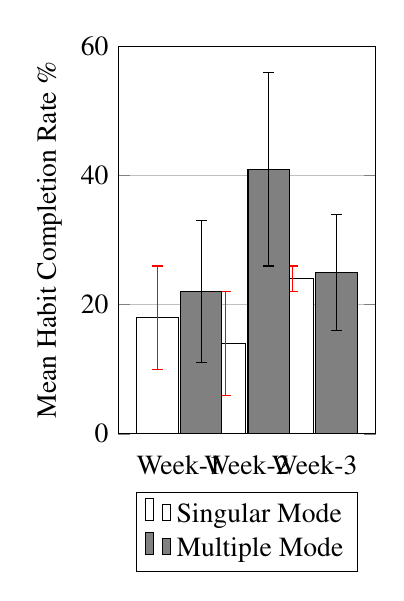
\begin{tikzpicture}
   \begin{axis}[
      width  = 0.4*\textwidth,
      height = 6.5cm,
      major x tick style = transparent,
      ybar=2*\pgflinewidth,
      bar width=15pt,
      ymajorgrids = true,
      symbolic x coords={Week-1, Week-2, Week-3},
      xtick = data,
      scaled y ticks = false,
      enlarge x limits=0.45,
      ymin=0,
      ymax=60,
      legend cell align=left,
      legend style={at={(0.5,-0.15)},anchor=north},
      ylabel={Mean Habit Completion Rate \%},
   ]
      \addplot[style={fill=white},error bars/.cd, y dir=both, y explicit,error bar style=red]
           coordinates { % Singular Modes
          (Week-1, 18)  += (0,8) -= (0,8)
          (Week-2, 14)  += (0,8) -= (0,8)
          (Week-3, 24)  += (0,2) -= (0,2)
      };

      \addplot[style={fill=gray},error bars/.cd, y dir=both, y explicit]
          coordinates { % Multiple Modes
          (Week-1, 22)  += (0,11) -= (0,11)
          (Week-2, 41)  += (0,15) -= (0,15)
          (Week-3, 25)  += (0,9) -= (0,9)
       };

      \legend{Singular Mode, Multiple Mode}

  \end{axis}
  \end{tikzpicture}
  \caption{Multiple vs. single-mode feedback on habit completion.}~\label{fig:habit_completion_3}
\end{figure}


\subsection{Habit Automaticity}
Participants completed habit automaticity questionnaires (SRBAI) at the end of week three and week four. Eleven participants completed both SRBAI questionnaires: two from the Audio condition, five from Visual, two from Audio-Visual and two from the control group.




\subsubsection{The effect of each condition on habit automaticity}
There was no statistically significant difference between scores as determined by a one-way ANOVA (see Figure~\ref{fig:habit_automaticity_1}) for SRBAI one ($F(3,7) = 0.333$, $p = 0.802$) and SRBAI two ($F(3,7) = 0.639$, $p = 0.614$). For each reward specifically a Tukey post hoc test revealed that there was no significant difference in scores for each reward.
% A paired-samples t-test was conducted on both questionnaires, showing a statistically significant increase in automaticity scores from week three (mean SRABI score = 14.18, SD = 3.78) to week four (mean = 15.09, SD = 4.34), $t(10) = 2.469$, $p$ $<$ $0.005$ (two-tailed). This meant that participant's habit automaticity did generally increase, as reported by a mean increase in SRBAI scores of 0.90 (CI = 95\%, from 0.08 to 1.72) and a large effect size as measured by $\eta^{2} = 0.37$.

\subsubsection{The effect of rewards on habit automaticity}
Comparing participants SRBAI results' with the control group shows the impact rewards had on automaticity (see Figure~\ref{fig:habit_automaticity_2}).
% An independent-samples t-test was conducted to compare both SRBAI one and SRBAI two for rewards and control (see Figure~\ref{fig:habit_automaticity_2}). For SRBAI one, there was also no significant differences in scores for rewards (mean = 14.33, SD = 3.84) and control (mean = 13.50, SD = 4.94; $t(9) = 0.224$, $p = 0.85$,
% two-tailed). The magnitude of the differences in the means (mean difference = 0.83,
% 95\% CI: \-29.43 to 27.76) was very small ($\eta^{2} = 0.005$). For SRBAI 2, there was no significant difference in scores for rewards
% (mean = 15.22, SD = 4.29) and control (mean = 14.50, SD = 6.36; $t(9) = 0.202$, $p = 0.84$,
% two-tailed). The magnitude of the differences in the means (mean difference = 0.72,
% 95\% CI: \-8.80 to 7.36) was very small ($\eta^{2} = 0.004$). Another test was conducted to validate this finding.
A one-way between-groups ANOVA with planned comparisons was conducted, but there was not a statistically significant difference for the two groups at SRBAI one: $F(1,9) = 0.02$, $p = 0.88$, and SRBAI two: $F(1,9) = 0.07$, $p = 0.78$. The difference in mean scores between the groups had, at SRBAI one: a medium effect with an effect size $\eta^{2} = 0.11$, and at SRBAI two: a large effect, with an effect size of $\eta^{2} = 0.17$.


\begin{figure}
  \centering
 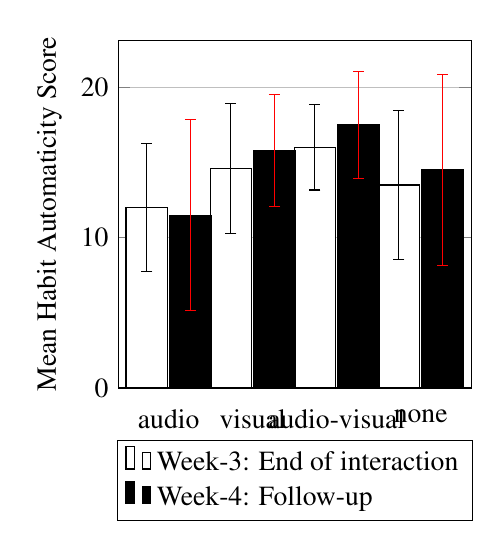
\begin{tikzpicture}
   \begin{axis}[
      width  = 0.5*\textwidth,
      height = 6cm,
      major x tick style = transparent,
      ybar=2*\pgflinewidth,
      bar width=15pt,
      ymajorgrids = true,
      symbolic x coords={audio, visual, audio-visual, none},
      xtick = data,
      scaled y ticks = false,
      enlarge x limits=0.2, % how far apart the bars are, the lower the further apart
      ymin=0,
      legend cell align=left,
      legend style={at={(0.5,-0.15)},anchor=north},
      ylabel={Mean Habit Automaticity Score},
   ]
      \addplot[style={fill=white},error bars/.cd, y dir=both, y explicit]
          coordinates {
          (audio, 12) += (0,4.243) -= (0,4.243)
          (visual, 14.6) += (0,4.336) -= (0,4.336)
          (audio-visual, 16) += (0,2.828) -= (0,2.828)
          (none, 13.5) += (0, 4.950) -= (0, 4.950)
          };

      \addplot[style={fill=black},error bars/.cd, y dir=both, y explicit,error bar style=red]
           coordinates {
          (audio, 11.5) += (0,6.364) -= (0,6.364)
          (visual, 15.8) += (0,3.701) -= (0,3.701)
          (audio-visual, 17.5) += (0,3.536) -= (0,3.536)
          (none, 14.5) += (0, 6.364) -= (0, 6.364)
           };

      \legend{Week-3: End of interaction, Week-4: Follow-up}

  \end{axis}
  \end{tikzpicture}
  \caption{The effect of each condition on habit automaticity.}~\label{fig:habit_automaticity_1}
\end{figure}


\begin{figure}
  \centering
 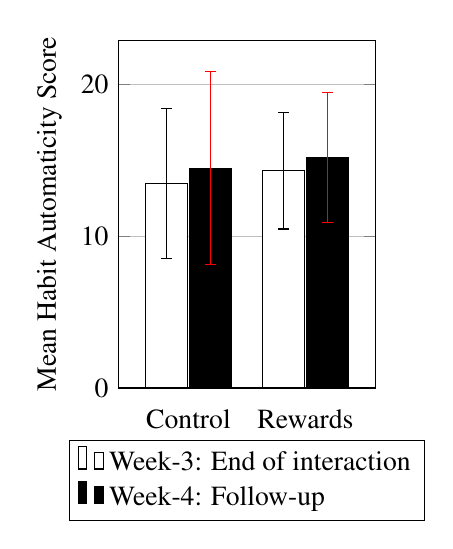
\begin{tikzpicture}
   \begin{axis}[
      width  = 0.4*\textwidth,
      height = 6cm,
      major x tick style = transparent,
      ybar=2*\pgflinewidth,
      bar width=15pt,
      ymajorgrids = true,
      symbolic x coords={Control,Rewards},
      xtick = data,
      scaled y ticks = false,
      enlarge x limits=0.60,
      ymin=0,
      legend cell align=left,
      legend style={at={(0.5,-0.15)},anchor=north},
      ylabel={Mean Habit Automaticity Score},
   ]
      \addplot[style={fill=white},error bars/.cd, y dir=both, y explicit]
          coordinates {
          (Control, 13.5) += (0,4.94) -= (0,4.94)
          (Rewards, 14.33) += (0,3.84) -= (0,3.84)
          };

      \addplot[style={fill=black},error bars/.cd, y dir=both, y explicit,error bar style=red]
           coordinates {
           (Control, 14.5) += (0,6.36) -= (0,6.36)
           (Rewards, 15.22) += (0,4.29) -= (0,4.29)
           };

      \legend{Week-3: End of interaction, Week-4: Follow-up}

  \end{axis}
  \end{tikzpicture}
  \caption{The effect of rewards on habit automaticity.}~\label{fig:habit_automaticity_2}
\end{figure}

\subsubsection{Multiple vs. single-mode feedback on habit automaticity}
To compare the effect audio-visual had on automaticity a one-way between-groups ANOVA with planned comparisons was conducted (see Figure~\ref{fig:habit_automaticity_3}). Participants were divided into two groups according to their reward condition. Group one: audio rewards and visual rewards and group two: audio-visual rewards. There was not a
statistically significant difference for the two groups at SRBAI one: $ F(1,9) = 1.04$, $p = 0.33$, and SRBAI two: $F(1,9) = 0.64$, $p = 0.44$. The difference in mean scores between the groups had, at SRBAI one: a medium effect with an effect size of $\eta^{2} = 0.11$, and at SRBAI two: a large effect, with an effect size of $\eta^{2} = 0.17$.


\begin{figure}
  \centering
 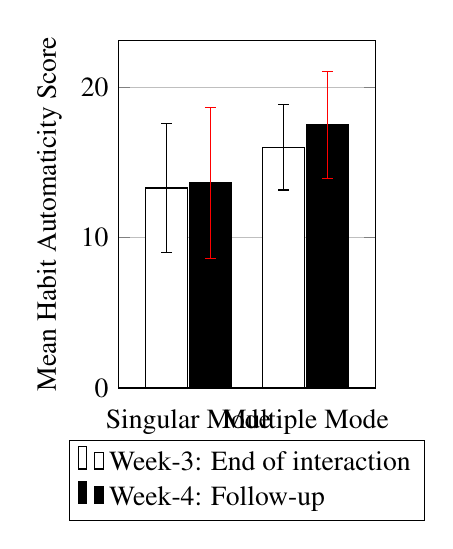
\begin{tikzpicture}
   \begin{axis}[
      width  = 0.4*\textwidth,
      height = 6cm,
      major x tick style = transparent,
      ybar=2*\pgflinewidth,
      bar width=15pt,
      ymajorgrids = true,
      symbolic x coords={Singular Mode, Multiple Mode},
      xtick = data,
      scaled y ticks = false,
      enlarge x limits=0.60,
      ymin=0,
      legend cell align=left,
      legend style={at={(0.5,-0.15)},anchor=north},
      ylabel={Mean Habit Automaticity Score},
   ]
      \addplot[style={fill=white},error bars/.cd, y dir=both, y explicit]
          coordinates {
          (Singular Mode, 13.3) += (0,4.289) -= (0,4.289)
          (Multiple Mode, 16) += (0,2.828) -= (0,2.828)
          };

      \addplot[style={fill=black},error bars/.cd, y dir=both, y explicit,error bar style=red]
           coordinates {
          (Singular Mode, 13.65) += (0,5.033) -= (0,5.033)
          (Multiple Mode, 17.5) += (0,3.536) -= (0,3.536)
           };

      \legend{Week-3: End of interaction, Week-4: Follow-up}

  \end{axis}
  \end{tikzpicture}
  \caption{Multiple vs. single-mode feedback on habit automaticity.}~\label{fig:habit_automaticity_3}
\end{figure}



\subsection{Interview Feedback}
Seven participants agreed to participate in optional interviews (their details are summarised in Table~\ref{table:transcript_participant_breakdown}). The interviews were recorded, transcribed and grouped into three themes: continuation with habit formation, attitudes towards rewards and attitudes towards the chatbot.

\begin{table}[b]
  \begin{tabular}{l l l l l l}
    \multicolumn{1}{l}{\small \textit{~}} &
    \multicolumn{1}{l}{\small \textit{Age}} & 
    \multicolumn{1}{l}{\small \textit{Gender}} & 
    \multicolumn{1}{l}{\small \textit{Condition}} &
    \multicolumn{1}{l}{\small \textit{Habit}} &
    \multicolumn{1}{p{1cm}}{\small \textit{Completion rate}} \\
    \midrule
    P1 & 24 & M & Visual & Meditation & 86\% \\
    P2 & 19 & F & Auditory & Stretch & 43\% \\ 
    P3 & 28 & F & Visual & Writing & 38\% \\
    P4 & 57 & F & No reward & Meditation & 80\% \\ 
    P5 & 25 & M & Visual & Meditation & 19\% \\ 
    P6 & 21 & F & No reward & Meditation & 33\% \\ 
    P7 & 32 & M & Visual-Auditory & Stretch & 90\% \\
  \end{tabular}
  \caption{Details of participants who were interviewed.}~\label{table:transcript_participant_breakdown}
\end{table}

\subsubsection{Continuation with habit completion}
When discussing the experiences with habit formation, we asked participants for their reasons of selecting their habits. P4 and P5 admitted choosing their habit because they had wanted to start that particular habit for a long time. P2 said that it was \textit{'not too much effort'} and P6 said it was \textit{'something successful people do'}. P7 wanted \textit{'to be more active'} P2 wanted a habit that was \textit{'less time consuming'}. Finally, P1, P5 and P6 wanted to \textit{'relieve stress'}. 

In terms of habit completion, while most participants were able to do it regularly, P6 reported always putting the message off and eventually their habit completion got \textit{'worse and worse'} until they stopped altogether. After the bot was removed, the same was true for all other interviewed participants, who admitted finding it difficult to continue with their habit. They \textit{'kept forgetting'} (P3), found it \textit{'harder to remember'} (P1) and lacked motivation, not performing the action if it had \textit{'been a long day'} (P5). P5 also tried to do it \textit{'every now and again'}, but usually they would only complete it if \textit{'they remembered'}. P1, P4, P6, and P7 all discussed not being able to remember to complete their habit after the bot was removed. This reveals the dependency between technology and habits, suggesting that the bot did not increase habit automaticity, or that the existing routine participants chose was not suitable for new habits, or that they were not given enough time to develop automaticity.

\subsubsection{Attitudes Towards Rewards}
Participants had mixed feelings about the rewards. Some \textit{'did not like the [visual] rewards'} (P1), skipping over them after the first few, they \textit{'just wanted to get rid of the notification dot'} (P1). Another participant (P3) said \textit{'some of them [audio-visual rewards] were funny'}, but they did not like them overall and mentioned the audio rewards were \textit{'too random'}. 

One participant (P5) thought the rewards did not give them an incentive towards their habit, just a \textit{'nice little extra'} and they discussed including time-sensitive rewards, as they did not want to listen to music before going to bed. This shows the importance of using an appropriate modality at particular times, e.g. not having audio rewards at certain times of the day. Finally, an upbeat participant (P7) talked about \textit{'always wanting to open them'} and \textit{'the combination was perfect'}. However, they said they also found them \textit{'repetitive'} (P7) and one participant stated that they simply wanted to get rid of the notification (P1). This implies that the bot was not tracking how many habits that participant completed, but instead how many times wanted the bot to stop messaging them.

\subsubsection{Attitudes Towards the Chatbot}
Participants were asked about the chatbot as the method of interaction. They found the method \textit{'pretty good'} (P2), they \textit{'liked it'} (P3) and \textit{'would have liked more interaction'} (P4). Some suggested expanding the bot with additional features, such as \textit{'help and support throughout'} (P4), \textit{'ideas on how to improve your habit'} (P4) and \textit{'advice on how to set aside time for your habit'} (P4). Others were neutral, some expecting \textit{'different messages, such as Hey [name], a bit more care about the person, a bit less like a robot'} (P7). 

Four participants (P2, P4, P6, P7) enjoyed the check-in notification aspect, but one found it \textit{'repetitive'} (P7) and \textit{'got annoying if I pressed Not Yet'} (P5). P1 and P3 wanted to see their progress as they tracked their habits, and talked about wanting to reflect on their data. They mentioned that they would feel \textit{'more encouraged to keep doing it, rather than random music [audio rewards]'} (P3). 

Six out of the seven participants wanted the prototype to come back with a few modifications (P1 was neutral): \textit{'enclosed with Fitbit so it is all in a single place'} (P2), \textit{'fine without rewards'} (P1, P3), \textit{'more interaction'} (P4) and \textit{'with statistics about my progress'} (P1, P3). Participants wanted the bot as more of a \textit{'constant persistent reminder'} (P6) with additional tracking elements to remind them to perform their habit to fit into their busy schedule. 

Five participants mentioned \textit{Headspace} – the popular meditation app (\url{www.headspace.com}), saying that they wanted a combination of the bot and meditation. It prompted one participant to download the Headspace app. Overall, participants wanted the bot to keep  track of their habit and they would use the Headspace app to help them perform their meditation.

Participants also gave additional, unexpected feedback by simply messaging the bot. They asked inquisitive questions, such as \textit{'what kind of thing are you looking to find out'} (P8), or provided feedback: \textit{'this is not working for me'} (P9). Others simply sent \textit{'stop'} (P10)) --- to try and stop the daily messages (the participant then blocked the bot). 

Negative comments towards the rewards and the bot were also expressed. When asked about being messaged every day, a participant sent this reply and then blocked the bot: \textit{'Do not do that, it will be annoying'} (P11), and another said \textit{'never message me'} (P12). Yet another posted that this was the \textit{'lame same band'} (P13) after receiving an audio reward.

\subsection{Summary}
Our results showed a statistically significant drop in habit completion for the control group without rewards. 
%This reveals the effect the rewards had on participant interaction with the bot and habit completion. 
The findings suggest that participants are more likely to complete their habit if given one of the rewards, especially if the reward is audio-visual. Participants with audio-visual rewards also had higher habit automaticity scores compared with only audio or only visual rewards; however, this difference was not statistically significant. Finally, participants picked habits they wanted to perform, but when the bot stopped notifying them, they lacked motivation to continue. Even though  participants enjoyed the rewards at the beginning, this passed and most participants reported disliking them after the first week. %Therefore, it is inconclusive whether the rewards or the combined modalities improved habit formation and automaticity.

\section{Discussion}
This research aimed to understand how different types of positive reinforcement -- audio, visual and audio-visual -- influence the process of habit formation, especially how they facilitate regular habit completion. We found that participants who received bot-delivered rewards completed more habits than the control group without rewards, which suggests that positive reinforcement delivered by a chatbot may have a better effect on habit completion than SMS reminders: in [REF] control group did better than positive reinforcement delivered by text messages.

There was also an increase in completed habits for participants with combined modalities when compared with the other reward modes. This matches existing literature for using multiple modalities to improve task completion rates~\cite{comparing_modalities_effects_of_visual_auditory, benefits_of_audio_visual_1, benefits_of_audio_visual_2, when_do_we_interact_multimodally,oussama_tap_the_shapetones}. Although during the interviews participants reported a drop in habit completion after removing the prototype, this is likely due to the lack of habit automaticity developed during the three week period~\cite{article_dont_kick_habit, article_realtime_feedback_improving_medication_taking}. Developing automaticity would enable the continuation of habit completion after one week without the prototype~\cite{article_beyond_self_tracking_designing_apps}.

Each individual reward did not have a significant effect on habit automaticity. Although participants with rewards had slightly higher automaticity scores, follow up interviews suggest that automaticity did not develop. A dependency could have been developed with the bot which would hinder habit automaticity~\cite{article_beyond_self_tracking_designing_apps}. Participants discussed negative feelings towards rewards during the interviews, however, participants attitudes towards interaction with the chatbot was mostly positive. All interviewed participants suggested features they would like, likely because the bot did not meet their needs. Moreover, each participant seemed to have mixed feelings towards the rewards. However, although the rewards did not significantly increase habit automaticity, they did improve the number of habits participants completed. Therefore, we can conclude that the chatbot has a potential as a tool for supporting habit formation. 

The prototype was based on the existing literature, i.e. it helped participants stick to a routine by reminding them of their routine and using positive reinforcement~\cite{positive_reinforcement_pro} and back up notifications~\cite{article_beyond_self_tracking_designing_apps}. However, because of the nature of interactions, participants might have treated the bot as a regular reminder. Therefore, the bot may have simply reinforced repetitive actions rather than facilitating the development of  automaticity~\cite{coaching_not_that_good}. 

%Finally, these findings are only impacted by the specific rewards used in this study delivered by the bot. Therefore, it is inconclusive whether audio-visual rewards in a general sense increase habit completion.


\subsection{Limitations and Future Work}
This research has a few key limitations that open up future work avenues. First, the small number of participants and the small sample of rewards used in the study make it unclear how these findings would generalise to other types of rewards with the same modality. Nevertheless, our findings already suggest a significant difference between combined modalities and singular to improve habit completion, which matches previous studies~\cite{benefits_of_audio_visual_1,benefits_of_audio_visual_2,comparison_of_auditory_visual_feedback} that compared of audio and visual modalities.

Second, the measurement of habit formation past the lifetime of the bot relied on the interviews. But only seven participants responded to the follow up interviews and their discussions relied on participants recall, which could be inaccurate. Future work conducting similar research with a larger sample size for the SRBAI questionnaire would validate the effect these rewards had on habit formation without the prototype.

Third, this research relies on participants self-reporting and some of them could have lied to remove the alert instead of performing the habit, just to get the reward. This is particularly true with the snooze function, as the voluntary interviews showed that some participants found the bot annoying and stopped using it over time. %These participants could have been simply getting rid of the back up notification rather than completing the habit, changing the measurement of how participants reacted to these back up notifications, instead of their habit. 
Therefore, it is difficult to draw any valid conclusion on actual habit performance. Future work into how quickly participants responded to the alerts and if the device delivery (browser or smartphone) affected these findings would allow us to better understand how participants interacted with the alerts.


% Using other motivating factors, such as streaks could have been better used to give insight to participants progress and challenged them to maintain it, using loss aversion~\cite{loss_aversion} to compare the impact of their broken streak with the gain of keeping it.
%Fourth, participants were able to personalise the chatbot with several different variable configurations. This personalisation could have effected the findings by not narrowing the condition variables. Replicating this research with tighter a configuration is needed to validate this line of reasoning. 
%[DON'T UNDERSTAND THIS ONE! ALSO, TOO MANY LIMITATIONS!]

Finally, future work could focus on comparing bot-delivered positive reinforcement to more traditional approaches, such as app notifications or  SMS. With their ease of implementation and access to a large pool of participants, chatbots are a promising platform for delivering behaviour change interventions. Further research into the effect of bot interactions on habit formation is needed to explore the full potential of this approach.   

\section{Conclusions}
We found that the type of reward did not influenced habit automaticity, but it nevertheless increased throughout the study. However, the rewards did improve the number of habits people completed, with the highest completion rates in the audio-visual condition, which suggests that bots may play a useful, albeit limited, role in supporting new behaviours. 
%We hope this research opens up new avenues for using bots as tools to help form new habits and give new behaviour change technology insights into positive reinforcement rewards from audio, visual and audio-visual modalities.

% -- FINDINGS --
% AUTOMATICITY
% Bot increased automaticity
% Specific rewards didn't increase automaticity

% COMPLETION
% Audio-Visual rewards then audio had highest completion increase
% Audio rewards had lowest

\section{Acknowledgements}
[Removed for peer review.]
% Thank you to all the participants involved who provided feedback throughout the study.

\balance{}

% % Either:
% %  1. Put \balance in the first column of the last page
% %  2. Don't use \balance
% %  3. hard-code a column break into the bbl file (before submission)
% % see more http://stackoverflow.com/questions/2149854/how-to-manually-equalize-columns-in-an-ieee-paper-if-using-bibtex
% \balance{}

\bibliographystyle{scaffold/SIGCHI-Reference-Format}
\bibliography{sample}
% \printbibliography

\end{document}
